\let\negmedspace\undefined
\let\negthickspace\undefined
\documentclass[journal]{IEEEtran}
\usepackage[a5paper, margin=10mm, onecolumn]{geometry}
%\usepackage{lmodern} % Ensure lmodern is loaded for pdflatex
\usepackage{tfrupee} % Include tfrupee package

\setlength{\headheight}{1cm} % Set the height of the header box
\setlength{\headsep}{0mm}     % Set the distance between the header box and the top of the text
\usepackage{xparse}
\usepackage{gvv-book}
\usepackage{gvv}
\usepackage{cite}
\usepackage{amsmath,amssymb,amsfonts,amsthm}
\usepackage{algorithmic}
\usepackage{graphicx}
\usepackage{textcomp}
\usepackage{xcolor}
\usepackage{txfonts}
\usepackage{listings}
\usepackage{enumitem}
\usepackage{mathtools}
\usepackage{gensymb}
\usepackage{comment}
\usepackage[breaklinks=true]{hyperref}
\usepackage{tkz-euclide} 
\usepackage{listings}
% \usepackage{gvv}                                        
\def\inputGnumericTable{} 
\usepackage[latin1]{inputenc}                                
\usepackage{color}                                            
\usepackage{array}                                            
\usepackage{longtable}                                       
\usepackage{calc}                                             
\usepackage{multirow}                                         
\usepackage{hhline}                                           
\usepackage{ifthen}                                           
\usepackage{lscape}

\begin{document}

\bibliographystyle{IEEEtran}
\vspace{3cm}

\title{GATE Questions 16}
\author{EE24BTECH11012 - Bhavanisankar G S}
% \maketitle
% \newpage
% \bigskip
{\let\newpage\relax\maketitle}
\begin{enumerate}
	\item The untimely loss of life is a cause of serious global concern as thousands of people get killed \underline{   } accidents every year while many others die \underline{   } diseases like cardio-vascular disease, cancer etc.
		\begin{enumerate}
				\begin{multicols}{2}
				\item in, of
				\item from, of
				\item during, from
				\item from, from
				\end{multicols}
		\end{enumerate}
	\item He was not only accused of theft \underline{   } of conspiracy.
		\begin{enumerate}
				\begin{multicols}{4}
				\item rather
				\item but also
				\item but even
				\item rather than
				\end{multicols}
		\end{enumerate}
	\item Select the word that fits the analogy : \\
		Explicit : Implicit :: Express : \underline{  }
		\begin{enumerate}
				\begin{multicols}{4}
				\item impress
				\item repress
				\item compress
				\item suppress
				\end{multicols}
		\end{enumerate}
	\item The Canadian constitution requires that equal importance be given to English and French. Lat year, Air Canada lost a lawsuit, and had to pay a six-figure fine to a Frenchspeaking couple after they filed complaints about formal in-flight announcements in English lasting 15 seconds, as opposed to informal 5 second messages in French. \\
		The French-speaking couple were upset at
		\begin{enumerate}
			\item the in-flight announcements being made in English.
			\item the English announcements being clearer than the French ones.
			\item the English announcements being longer than the French ones.
			\item equal importance being given to English and French.
		\end{enumerate}
	\item A superadditive function $f( )$ satisfies the following property
		$$ f(x_1 + x_2) \geq f(x_1) + f(x_2) $$
		Which of the following functions is a superadditive function for $x \geq 1$ ?
		\begin{enumerate}
				\begin{multicols}{4}
				\item $e^x$
				\item $\sqrt{x}$
				\item $\frac{1}{x}$
				\item $e^{-x}$
				\end{multicols}
		\end{enumerate}
	\item The global financial crisis in 2008 is considered to be the most serious world-wide financial crisis, which started with the subprime lending crisis in USA in 2007. The sub-prime lending crisis led to the banking crisis in 2008 with the collapse of Lehman Brothers in 2008. The sub-prime lending refers to the provision of loans to those borrowers who may have difficulties in repaying loans, and it arises because of excess liquidity following the East Asian crisis. \\
		Which one of the following sequences shows the correct precedence as per the given passage ?
		\begin{enumerate}
			\item East Asian crisis $\rightarrow$ sub-prime lending crisis $\rightarrow$ banking crisis $\rightarrow$ global financial crisis
			\item Sub-prime lending crisis $\rightarrow$ global financial crisis $\rightarrow$ banking crisis $\rightarrow$ East Asian crisis
			\item Banking crisis $\rightarrow$ sub-prime lending crisis $\rightarrow$ global financial crisis $\rightarrow$ East Asian crisis
			\item Global financial crisis $\rightarrow$ East Asian crisis $\rightarrow$ banking crisis $\rightarrow$ sub-prime lending
		\end{enumerate}
	\item It is quarter past three in your watch. The angle between the hour hand and the minute hand is \underline{  }
		\begin{enumerate}
				\begin{multicols}{4}
				\item $0 \degree$
				\item $7.5 \degree$
				\item $ 15 \degree$
				\item $22.5 \degree$
				\end{multicols}
		\end{enumerate}
	\item A circle with centre O is shown in the figure. A rectangle PQRS of maximum possiblr area is inscribed in the circle. If the radius of the circle is $a$, then the area of the outer portion is \underline{  }
		\begin{figure}[H]
	\centering
	\begin{circuitikz}
\tikzstyle{every node}=[font=\normalsize]
\draw  (4.75,12.75) circle (2.75cm);
\draw  (2.5,14.5) rectangle (7,11.25);
\draw [short] (4.75,12.75) -- (2.5,11.25);
\node [font=\LARGE] at (2.25,14.75) {P};
\node [font=\LARGE] at (2.25,11) {S};
\node [font=\LARGE] at (7.5,14.75) {Q};
\node [font=\LARGE] at (7.5,11) {R};
\node [font=\LARGE] at (5,12.75) {O};
\node [font=\normalsize] at (3.5,12.25) {a};
\end{circuitikz}
	\label{}
	%\caption{}
\end{figure}

		\begin{enumerate}
				\begin{multicols}{2}
				\item $\pi a^2 - a^2$
				\item $\pi a^2 - \sqrt{2} a^2$
				\item $\pi a^2 - 2 a^2$
				\item $\pi a^2 - 3a^2$
				\end{multicols}
		\end{enumerate}
	\item $a, b \text{and} c$ are real numbers. The quadratic equation $ax^2 + bx + c = 0 $ has equal roots, which is $\beta$, then
		\begin{enumerate}
				\begin{multicols}{2}
				\item $\beta = \frac{b}{a}$
				\item $\beta ^2 = ac$
				\item $\beta ^3 = \frac{bc}{2a^2}$
				\item $b^2 \neq 4ac$
				\end{multicols}
		\end{enumerate}
	\item The following figure shows the data of students enrolled in 5 years ( 2014 to 2018 ) for two schools P and Q. During this period, the rario of the average number of the srudets enrolled in school P to the average of the difference of the number of students enrolled in schools P and Q is \underline{  }
		\begin{figure}[H]
			\begin{tikzpicture}
  \draw[->] (0,0) -- (0,7) node[above] {Profit percentage} ;
  \draw[->] (0,0) -- (10,0) node[right] {Year} ;

  \draw[fill=red] (1.25,0) rectangle (1.5,1) ;
  \draw[fill=blue] (1.5,0) rectangle (1.75,2) ;
  \draw[fill=red] (2.25,0) rectangle (2.5,2) ;
  \draw[fill=blue] (2.5,0) rectangle (2.75,3) ;
  \draw[fill=red] (3.25,0) rectangle (3.5,4) ;
  \draw[fill=blue] (3.5,0) rectangle (3.75,3) ;
  \draw[fill=red] (4.25,0) rectangle (4.5,4) ;
  \draw[fill=blue] (4.5,0) rectangle (4.75,5) ;
  \draw[fill=red] (5.25,0) rectangle (5.5,5) ;
  \draw[fill=blue] (5.5,0) rectangle (5.75,6) ;
  \draw[fill=red] (6.25,0) rectangle (6.5,4) ;
  \draw[fill=blue] (6.5,0) rectangle (6.75,6) ;

  \draw[fill=red] (0.9,5.9) rectangle (1.1,6.1) ;
  \draw[fill=blue] (0.9,6.5) rectangle (1.1,6.7) ;
	\node at (2.2,6.6) {Company Q} ;
	\node at (2.2,6) {Company P} ;

  \node at (1.25,-0.5) {2013} ;
  \node at (2.25,-0.5) {2014} ;
  \node at (3.25,-0.5) {2015} ;
  \node at (4.25,-0.5) {2016} ;
  \node at (5.25,-0.5) {2017} ;
  \node at (6.25,-0.5) {2018} ;
  \node at (-0.5,1) {10} ;
  \node at (-0.5,2) {20} ;
  \node at (-0.5,3) {30} ;
  \node at (-0.5,4) {40} ;
  \node at (-0.5,5) {50} ;
  \node at (-0.5,6) {60} ;
  \node at (-0.5,7) {70} ;

  
\end{tikzpicture}



		\end{figure}
		\begin{enumerate}
				\begin{multicols}{4}
				\item 8:23
				\item 23:8
				\item 23:31
				\item 31:23
				\end{multicols}
		\end{enumerate}
	\item For $f(x) = \abs{x}$ with $\frac{df}{dx}$ denoting the derivative, the mean value theorem is not applicable because
		\begin{enumerate}
			\item $f(x)$ is not continuous at $x=0$
			\item $f(x) = 0$ at $x=0$
			\item $\frac{df}{dx}$ at $x=0$
			\item $\frac{df}{dx}$ is not defined at $x=0$
		\end{enumerate}
	\item For the function $f(x) = \frac{e^{-\lambda}}{2 \sigma^2 \sqrt{2 \pi}}, \text{where} \lambda = \frac{1}{2 \sigma^2} \brak{x - \mu}^2 $, and $\sigma$ and $\mu$ are constants, the maximum occurs at
		\begin{enumerate}
				\begin{multicols}{4}
				\item $x = \sigma$
				\item $x = \sigma \sqrt{2 \pi}$
				\item $x = 2 \sigma^2$
				\item $x = \mu$
				\end{multicols}
		\end{enumerate}
	\item $y = Ae^{mx} + Be^{-mx}$, where $A, B \text{and} m$ are consttants, is a solution of
		\begin{enumerate}
				\begin{multicols}{2}
				\item $\frac{d^2y}{dx^2} - m^2y = 0$
				\item $A \frac{d^2y}{dx^2} + m^2y = 0$
				\item $B \frac{d^2y}{dx^2} + Ay = 0$
				\item $\frac{d^2y}{dx^2} + my = m^2$
				\end{multicols}
		\end{enumerate}
\end{enumerate}
\end{document}

